\documentclass[border=4pt]{standalone}
\usepackage{amsmath,amssymb}
\usepackage{tikz}
\usetikzlibrary{arrows.meta,calc,decorations.pathreplacing,patterns,shapes.geometric,positioning,shadings,decorations.markings,decorations.pathmorphing}

\begin{document}
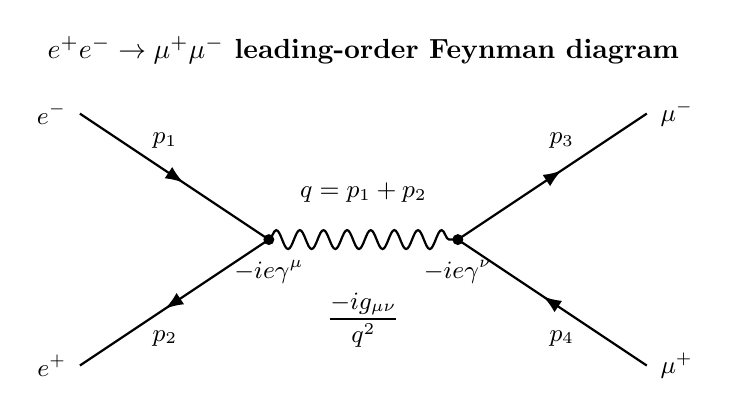
\begin{tikzpicture}[
  font=\small,
  fermion/.style={thick, decoration={markings, mark=at position 0.55 with {\arrow{Latex}}}, postaction={decorate}},
  photon/.style={thick, decorate, decoration={snake, amplitude=1.2mm, segment length=3mm}},
  vertex/.style={circle, fill=black, inner sep=1.4pt}
]

% --- coordinates ---
\coordinate (eIn1) at (-3.6, 1.6);   % e^- incoming
\coordinate (eIn2) at (-3.6,-1.6);   % e^+ incoming
\coordinate (V1)   at (-1.2, 0);     % left vertex
\coordinate (V2)   at ( 1.2, 0);     % right vertex
\coordinate (mOut1) at ( 3.6, 1.6);  % mu^- outgoing
\coordinate (mOut2) at ( 3.6,-1.6);  % mu^+ outgoing

% --- electron / positron incoming lines (arrows toward vertex) ---
\draw[fermion] (eIn1) -- (V1);
\draw[fermion] (V1) -- (eIn2);

% --- muon outgoing lines (arrows away from vertex) ---
\draw[fermion] (V2) -- (mOut1);
\draw[fermion] (mOut2) -- (V2);

% --- virtual photon (wavy line) ---
\draw[photon] (V1) -- (V2);

% --- vertices ---
\node[vertex] at (V1) {};
\node[vertex] at (V2) {};

% --- particle labels at external legs ---
\node[anchor=east] at ($(eIn1)+(-0.05,0)$) {$e^{-}$};
\node[anchor=east] at ($(eIn2)+(-0.05,0)$) {$e^{+}$};
\node[anchor=west] at ($(mOut1)+(0.05,0)$) {$\mu^{-}$};
\node[anchor=west] at ($(mOut2)+(0.05,0)$) {$\mu^{+}$};

% --- momentum labels ---
\node[above] at ($(eIn1)!0.45!(V1)+(0,0.15)$) {$p_{1}$};
\node[below] at ($(eIn2)!0.45!(V1)+(0,-0.15)$) {$p_{2}$};
\node[above] at ($(V2)!0.55!(mOut1)+(0,0.15)$) {$p_{3}$};
\node[below] at ($(V2)!0.55!(mOut2)+(0,-0.15)$) {$p_{4}$};
\node[above] at ($(V1)!0.5!(V2)+(0,0.35)$) {$q = p_{1}+p_{2}$};

% --- vertex factor labels ---
\node[below=4pt of V1] {$-ie\gamma^{\mu}$};
\node[below=4pt of V2] {$-ie\gamma^{\nu}$};

% --- propagator label ---
\node[below] at ($(V1)!0.5!(V2)+(0,-0.55)$) {$\dfrac{-ig_{\mu\nu}}{q^{2}}$};

% --- title-style header at top ---
\node[align=center, font=\bfseries] at (0, 2.4) {$e^{+}e^{-}\to \mu^{+}\mu^{-}$ leading-order Feynman diagram};

\end{tikzpicture}
\end{document}
